\documentclass{article}
\usepackage{hyperref}
\usepackage{amsmath}
\usepackage{amssymb}
\usepackage{pgfplots}
\usepackage{float}
\usepackage{todonotes}
\usepackage{tikz}
\usepackage[shortlabels]{enumitem}

\renewcommand{\Re}{\mathbb{R}}
\newcommand{\Li}{\mathcal{L}}
\newcommand{\Ex}{\mathbb{E}}
\renewcommand{\Pr}{\mathbb{P}}
\newcommand{\Hy}{\mathcal{H}}
\newcommand{\sign}{\text{sign}}
\newcommand{\error}{\text{error}}

\newcommand\bigO[1]{
    \ensuremath{\mathcal{O}\left(#1\right)}
    }

\newcommand{\sigmoidPlot}{
    
    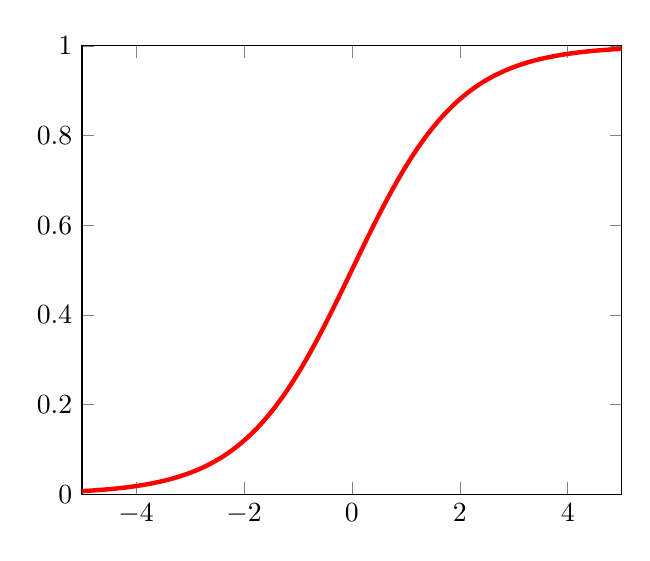
\begin{tikzpicture}
        \begin{axis}[xmin=-5, xmax=5, ymin=0, ymax=1, samples=150]
        \addplot[red, ultra thick] {1/(1+exp(-x))};
        \end{axis}
    \end{tikzpicture}
    
    }

\usetikzlibrary{positioning, calc}
\usetikzlibrary{arrows.meta}

\tikzstyle{circlebox}=[circle,thick,draw=black!75,minimum size=8mm]
\tikzstyle{inputnode}=[circlebox, draw=blue!75]
\tikzstyle{hiddennode}=[circlebox, draw=orange!75]
\tikzstyle{outputnode}=[circlebox, draw=orange!75]
\tikzstyle{simplebox}=[rectangle,thick,draw=black!75,
fill=black!20,minimum size=4mm]
\tikzstyle{textbox}=[rectangle,thick,minimum size=4mm,draw=black!0,
fill=black!0]
\tikzstyle{halfvdistance}=[yshift=-0.7cm]
\tikzstyle{abovebetween}=[xshift=-2.7mm]
\tikzstyle{edgepath} = [-Latex,->,shorten >=1pt,-stealth,semithick, rounded 
corners=5pt]

\def \nodedv {0.735cm}
\def \nodedh {0.65cm}

\tikzset{
    between/.style args={#1 and #2}{
        at = ($(#1)!0.5!(#2)$)
    }
}

\begin{document}
    \section{Subjects}
    \begin{itemize}
        \item Backpropagation
        \item Deep Nets
        \item PCA
        \item Autoencoder
    \end{itemize}
    
    \section{Notes}
    
    \subsection{Neurons and background}
    Neurons consist of a dendritic tree (the input, which branches a lot), the 
    axon (the output, which branches a little bit) and the cell body with 
    nucleus.
    
    Neurons work by having axons connected to dendritic trees, they give a 
    binary ($0$ or $1$) output, after an axon has sent a $1$, it has to 
    recharge.
    
    In order to model this, we've got binary input $x_1,\dots, x_n$ which is 
    sent to the nucleus that sums the inputs together and outputs $1$ if the 
    input exceeds some threshold.
    
    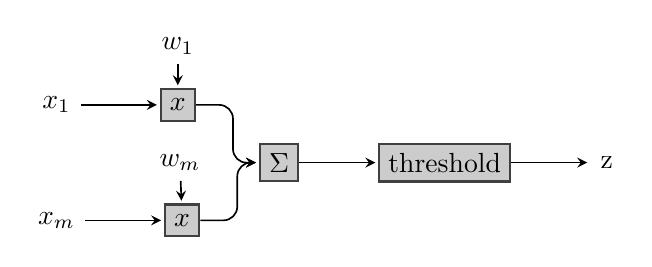
\begin{tikzpicture}
        \node[textbox] (x11) {$x_1$};
        \node[simplebox, right=of x11] (n1) {$x$};
        \node[textbox, above=of n1, halfvdistance] (w1) {$w_1$};
        \path[edgepath]
            (x11) edge node {} (n1)
            (w1) edge node {} (n1);
            
        \node[textbox, below=of x11] (x1m) {$x_m$};
        \node[simplebox, right=of x1m] (nm) {$x$};
        \node[textbox, between=nm and n1] (wm) {$w_m$};
        
        \node[simplebox, right=of n1, between=nm and n1] (sigma1) {$\Sigma$};
        \node[simplebox, right=of sigma1] (threshold1) {threshold};
        \node[textbox, right=of threshold1] (z) {z};
        
        \draw[edgepath]
            (x1m) edge node {} (nm)
            (wm) edge node {} (nm)
            (sigma1) edge node {} (threshold1)
            (threshold1) edge node {} (z);
        \draw[edgepath]
            (n1) -| ++(0.7cm,-\nodedv) -- (sigma1);
        \draw[edgepath]
            (nm) -| ++(0.7cm,\nodedv) -- (sigma1);
    \end{tikzpicture}
    
    This models the following properties:
    \begin{itemize}
        \item All or non
        \item Cumulative influence
        \item Synaptic weight
    \end{itemize}
    But there are more properties that we might like to model, like:
    \begin{itemize}
        \item Refractory period, recovery time of each neuron.
        \item Axonal bifurcation, each pulse will either go down one branch of 
        the axon or the other.
        \item Time patterns, we don't know if the timing of when impulses hit 
        neurons matters.
    \end{itemize}
    So we actually don't know if what we are modelling is the essence of how 
    neurons work or not. But we will start with the simple model.
    
    If we look at what a neural net actually is, then it's a vector of input 
    that goes through a ``box'' which uses some weights and threshold and then 
    outputs some vector $z$. Formally: $z = f(x,w,t)$. So the neural network is 
    just the function $f$, when we train the neural net, all we need to do is 
    change the weights and threshold. We can also think of the neural net as a 
    ``function approximator''.
    
    So, how do we measure the performance of the neural network? If we say the 
    desired result of the neural net $d$ is the function $g$ on the input 
    $x$, $d=g(x)$, then it would be natural to define the performance as: 
    $P=\|d-z\|$, this turns out to be mathematically inconvenient so instead we 
    will use the performance indicator: $P=\|d-z\|^2$.
    
    What we want to do, is of course to maximize the performance. We can do 
    this using gradient descent, for example for the weights $w_1$ and $w_2$:
    \begin{equation*}
        \Delta w= \eta \left(\frac{\partial P}{\partial w_1}i+\frac{\partial 
        P}{\partial w_2}j\right)
    \end{equation*}
    Unfortunately, the function is not linear, and thus gradient descent 
    doesn't really work. This was an issue for a long time untill Paul Werbos 
    figure it out.
    
    First of all, those thresholds are annoying as they are just extra baggage, 
    so we would like to reduce $z$ to be a function of just the inputs and 
    weights:
    \begin{equation*}
        z=f(x,w)
    \end{equation*}
    So what he proposed instead, was adding the bias input to each neuron $w_0$ 
    which is always set to $1$.
    
    
    \begin{tikzpicture}
    \node[textbox, right=of n1, abovebetween] (w0) {$w_0$};
    \node[textbox, right=of w0, yshift=0.5cm, xshift=-0.5cm] (b1) {$1$};
    
    \node[textbox] (x11) {$x_1$};
    \node[simplebox, right=of x11] (n1) {$x$};
    \node[textbox, above=of n1, halfvdistance] (w1) {$w_1$};
    \path[edgepath]
    (x11) edge node {} (n1)
    (w1) edge node {} (n1);
    
    \node[textbox, below=of x11] (x1m) {$x_m$};
    \node[simplebox, right=of x1m] (nm) {$x$};
    \node[textbox, between=nm and n1] (wm) {$w_m$};
    
    \node[simplebox, right=of n1, between=nm and n1] (sigma1) 
    {$\Sigma$};
    \node[simplebox, right=of sigma1] (threshold1) {threshold};
    \node[textbox, right=of threshold1] (z) {z};
    
    \draw[edgepath]
    (x1m) edge node {} (nm)
    (wm) edge node {} (nm)
    (sigma1) edge node {} (threshold1)
    (threshold1) edge node {} (z)
    (b1) edge node {} (w0);
    \draw[edgepath]
        (n1) -| ++(\nodedh,-\nodedv) -- (sigma1);
    \draw[edgepath]
        (nm) -| ++(\nodedh,\nodedv) -- (sigma1);
    \draw[edgepath]
        (w0) -| ++(-\nodedh,-\nodedv) -- (sigma1);
    \end{tikzpicture}
    And then we let $w_0=\text{threshold}$, then the threshold is effectively 
    $1$.\todo{revisit}
    
    Step two, is to smooth the threshold function, which we could do by 
    applying the sigmoid function $\sigma(\alpha)=\frac{1}{1+e^{-\alpha}}$. 
    Then it will be $1$ if $\alpha$ is very big, and $0$ if $\alpha$ is very 
    small.
    \sigmoidPlot
    The generalized term ``activation function'' $\phi$ is in this case 
    $\sigma$, our 
    function is linear and we can take the partial derivatives to the 
    function. Now, suppose we have a very simple neural network:
    
    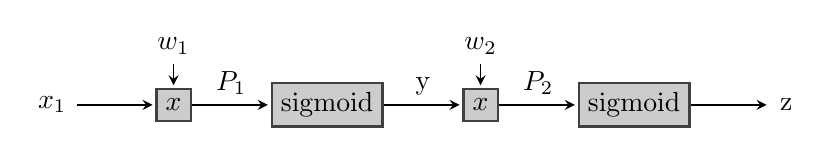
\begin{tikzpicture}
    \node[textbox] (x11) {$x_1$};
    \node[simplebox, right=of x11] (n1) {$x$};
    \node[textbox, above=of n1, halfvdistance] (w1) {$w_1$};
    \node[simplebox, right=of n1] (sigmoid1) {sigmoid};
    
    \path[edgepath]
        (x11) edge node {} (n1)
        (w1) edge node {} (n1)
        (n1) edge node[above] {$P_1$} (sigmoid1);
        
        
    \node[simplebox, right=of sigmoid1] (n2) {$x$};
    \node[textbox, above=of n2, halfvdistance] (w2) {$w_2$};
    \node[simplebox, right=of n2] (sigmoid2) {sigmoid};
    
    \path[edgepath]
        (sigmoid1) edge node[above] {y} (n2)
        (w2) edge node {} (n2)
        (n2) edge node[above] {$P_2$} (sigmoid2);
        
    \node[textbox, right=of sigmoid2] (z) {z};
    
    \path[edgepath]
        (sigmoid2) edge node {} (z);
    \end{tikzpicture}
    
    Now we want to re-write the partial derivative using the chain rule:
    \begin{equation*}
        \frac{\partial P}{\partial w_2} = \frac{\partial P}{\partial z} 
        \frac{\partial z}{\partial w_2} = \frac{\partial P}{\partial z} 
        \frac{\partial z}{\partial p_2} \frac{\partial p_2}{\partial w_2} 
    \end{equation*}
    We can do the same thing for $w_2$:
    \begin{equation*}
        \frac{\partial P}{\partial w_1} = \frac{\partial P}{\partial z} 
        \frac{\partial z}{\partial p_2} \frac{\partial p_2}{\partial y} 
        \frac{\partial y}{\partial p_1} \frac{\partial p_1}{\partial w_1} 
    \end{equation*}
    We can rewrite these two products as:
    \begin{align*}
        \frac{\partial P}{\partial w_2}&= \frac{\partial p_2}{\partial w_2} 
        \frac{\partial z}{\partial p_2} \frac{\partial P}{\partial z}\\
        \frac{\partial P}{\partial w_1}&=\frac{\partial p_1}{\partial w_1} 
        \frac{\partial y}{\partial p_1} \frac{\partial p_2}{\partial y} 
        \frac{\partial z}{\partial p_2} \frac{\partial P}{\partial z}
    \end{align*}
    Now we can compute the derivatives, in this example, the resulting 
    performance $P$ is: 
    \begin{equation*}
    P=\frac{1}{2}(d-z)^2
    \end{equation*}
    And thus we can compute
    \begin{equation*}
        \frac{\partial P}{\partial w_2}= \frac{\partial p_2}{\partial w_2} 
        \frac{\partial z}{\partial p_2} (d-z)
    \end{equation*}
    $p_2$ is simply $p_2 w_2$ so we get:
    \begin{equation*}
        \frac{\partial P}{\partial w_2}= y 
        \frac{\partial z}{\partial p_2} (d-z)
    \end{equation*}
    Finally the derivative of the sigmoid function is simple:
    \begin{equation*}
    \frac{\partial P}{\partial w_2}= y 
    (1-\sigma(\alpha))\sigma(\alpha) (d-z)
    \end{equation*}
    In this case the output of the $\sigma$ is $z$ so:
    \begin{equation*}
    \frac{\partial P}{\partial w_2}= y 
    (1-z)z (d-z)
    \end{equation*}
    Now if we look at the derivative for $\frac{\partial P}{\partial w_1}$, it 
    turns out that the last two elements we needed to compute, was the same as 
    the last two elements in the computation of $\frac{\partial P}{\partial 
    w_2}$! So if we make a neural network, where each ``column of neurons'' or 
    layer is densely connected, i.e. each output from the previous layer 
    connects to each input from the next layer, then even though the amount of 
    connections increases exponentially, the computation of the derivatives do 
    not! 
    
    The thing to note here, is that the output of layer $i$ has to go through 
    layer $i+1$ in order to affect the performance indicator. So the derivative 
    for layer $i$ can re-use computation from the derivative of $i+1$. So the 
    amount of work we are gonna have to do will be:
    \begin{itemize}
        \item Linear in depth
        \item With respect to width it, it will be proportional to the number 
        of connections and thus depends on $w^2$
    \end{itemize}
    
    This is the foundation for the backpropagation algorithm, and why neural 
    networks can efficiently learn.
    
    \subsection{Notation}
    \begin{itemize}
        \item $n_l$ is the number of layers.
        \item $s_l$ is the number of nodes in layer $l$ (not counting the bias 
        unit)
        \item $L_l$ is layer $l$.
        \item $L_0$ is the input layer, $L_{n_l}$ is the output layer
        \item $W_{ij}^{(l)}$ is the weight associated with the connection 
        between unit $j$ in layer $l$ and unit $i$ in layer $l+1$
        \item $b_i^{(l)}$ is the bias associated with unit $i$ in layer $l+1$
        \item $a_i^{(l)}$ is the activation (or the output value) of unit $i$ 
        in layer $l$. For $l=1$ we use $a_i^{(1)}=x_i$
        \item $z_i^{(l)}=\sum_{j=1}^{n}W_{ij}^{(l)}x_j+b_i^{(l)}$ is a 
        convenience notation such that $a_i^{(l)}=\phi(z_i^{(l)})$
    \end{itemize}
    
    Let's look at this example network:
    
    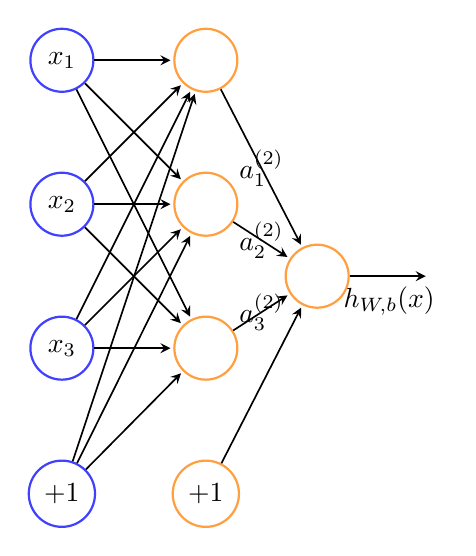
\begin{tikzpicture}
    \node[inputnode] (x1) {$x_1$};
    \node[inputnode, below=of x1] (x2) {$x_2$};
    \node[inputnode, below=of x2] (x3) {$x_3$};
    \node[inputnode, below=of x3] (b1) {$+1$};
    
    \node[hiddennode, right=of x1] (h1) {};
    \node[hiddennode, below=of h1] (h2) {};
    \node[hiddennode, below=of h2] (h3) {};
    \node[hiddennode, below=of h3] (b2) {$+1$};
    
    \node[outputnode, right=of h1, between=h2 and h3] (o1) {};
    \node[right=of o1] (o) {};
    
    \path[edgepath]
        (x1) edge node {} (h1)
        (x1) edge node {} (h2)
        (x1) edge node {} (h3)
        (x2) edge node {} (h1)
        (x2) edge node {} (h2)
        (x2) edge node {} (h3)
        (x3) edge node {} (h1)
        (x3) edge node {} (h2)
        (x3) edge node {} (h3)
        (b1) edge node {} (h1)
        (b1) edge node {} (h2)
        (b1) edge node {} (h3)
        (h1) edge node {$a_1^{(2)}$} (o1)
        (h2) edge node {$a_2^{(2)}$} (o1)
        (h3) edge node {$a_3^{(2)}$} (o1)
        (b2) edge node {} (o1)
        (o1) edge node[below] {$h_{W,b}(x)$} (o);
    \end{tikzpicture}
    
    This neural network represents the following computation:
    \begin{align*}
        a_1^{(2)} &= 
        \phi\left(W_{11}^{(1)}x_1+W_{12}^{(1)}x_2+W_{13}^{(1)}x_3+b_1^{(1)}\right)\\
        a_2^{(2)} &= 
        \phi\left(W_{21}^{(1)}x_1+W_{22}^{(1)}x_2+W_{23}^{(1)}x_3+b_2^{(1)}\right)\\
        a_3^{(2)} &= 
        \phi\left(W_{31}^{(1)}x_1+W_{32}^{(1)}x_2+W_{33}^{(1)}x_3+b_3^{(1)}\right)\\
        h_{W,b}(x) &= 
        a_1^{(3)}=\phi\left(W_{11}^{(2)}a_1^{(2)}+W_{12}^{(2)}a_2^{(2)}+W_{13}^{(2)}a_3^{(2)}\right)
    \end{align*}
    
    If we extend the activation function, to work on vectors such that 
    $f([z_1,z_2,z_3])=\left[f(z_1), f(z_2), f(z_3)\right]$ then we can write 
    the previous equation in a more compact fashion:
    \begin{align*}
        z^{(2)}&=W^{(1)}x+b^{(1)}\\
        a^{(2)}&=\phi\left(z^{(2)}\right)\\
        z^{(3)}&=W^{(2)}a^{(2)}+b^{(2)}\\
        h_{W,b}(x)&=a^{(3)}=\phi\left(z^{(3)}\right)
    \end{align*}
    Which can be generalized to:
    \begin{align*}
        z^{(l+1)}&=W^{(l)}a^{(l)}+b^{(l)}\\
        a^{(l+1)}&=\phi\left(z^{(l+1)}\right)
    \end{align*}
    
    The most common neural networks, are $n_l$-layered networks where $L_1$ is 
    the input, $L_{n_l}$ the output and $L_i$ is densely connected to 
    $L_{i+1}$. In order to compute the output, we would simply have to compute 
    the activation of $L_2$, $L_3$ etc. up to layer $L_{n_l}$, this is an 
    example of a \textbf{feedforward} neural network, as there are no loops or 
    cycles.
    
    \subsection{Backpropagation}
    Suppose we have a training set $D = \{(x_1,y_1),\dots,(x_m,y_m)\}$, we can 
    then train our neural network with batch gradient descent, with the cost 
    function for single sample as:
    \begin{equation*}
        J(W,b;x,y)=\frac{1}{2}\|h_{W,b}(x)-y\|^2
    \end{equation*} 
    This is simply a (one-half) squared-error cost function. The overall cost 
    function is then defined to be:
    \begin{equation*}
        J(W,b) = 
        \frac{1}{|D|}\sum_{i=1}^{|D|}\left(\frac{1}{2}\|h_{W,b}(x_i)-y_i\|^2\right)
    \end{equation*}
    If we add a weight decay term for regularization, then it becomes:
    \begin{equation*}
        J(W,b)=\frac{1}{|D|}\sum_{i=1}^{|D|}\left(\frac{1}{2}\|h_{W,b}(x_i)-y_i\|^2\right)
        + \frac{\lambda}{2} 
        \sum_{l=1}^{n_l-1}\sum_{i=1}^{s_l}\sum_{j=1}^{s_{l+1}}\left(W_{ji}^{(l)}\right)^2
    \end{equation*}
    Our goal now, is to minimize $J(W,b)$. To train our neural network, we will 
    initialize each parameter $W_{ij}^{(l)}$ and each $b_i^{(l)}$ to a small 
    random value near zero. If they are all the same value (e.g. $0$) then they 
    will end up learning the same function such that 
    $a_1^{(2)}=a_2^{(2)}=a_3^{(2)}=\dots$ for any input $x$.
    
    Each iteration of gradient descent then updates the parameters $W,b$ as 
    follows:
    \begin{align*}
        W_{ij}^{(l)}&=W_{ij}^{(l)}-\eta \frac{\partial}{\partial 
        W_{ij}^{(l)}}J(W,b)\\
        b_i^{(l)}&=-\eta \frac{\partial}{\partial b_i^{(l)}}J(W,b)
    \end{align*}
\end{document}